\section{Supplemental Material}

\subsection{One-Max Task}
\label{sec:one-max}

We used the one-max task for population size and genealogical inference experiments.
This task selects over binary string of length 100 for the number of 1's set.
Fitness preferred individuals with more 1's over individuals with fewer.
Population size was 200, initialized randomly.
In treatments where population size decreased during an evolutionary run, excess individuals were designated for elimination randomly.
In treatments where population size increased during an evolutionary run,
new population slots were filled through selection over the existing population.

Selection was performed using tournament selection with synchronous generations.
Default tournament size was 2.
Evolutionary runs lasted 100 generations.
Two-point crossover (mating) and bit-flip mutation with per-bit probability 0.05 each generation prior to selection.
Operator choice and parameter selections follows one-max example code from the DEAP package \citep{fortin2012deap}.

\subsection{Population Size Inference Example}
\label{sec:population-size-inference-example}

\begin{figure}
  \centering

  \begin{minipage}{.65\textwidth}
    \centering
    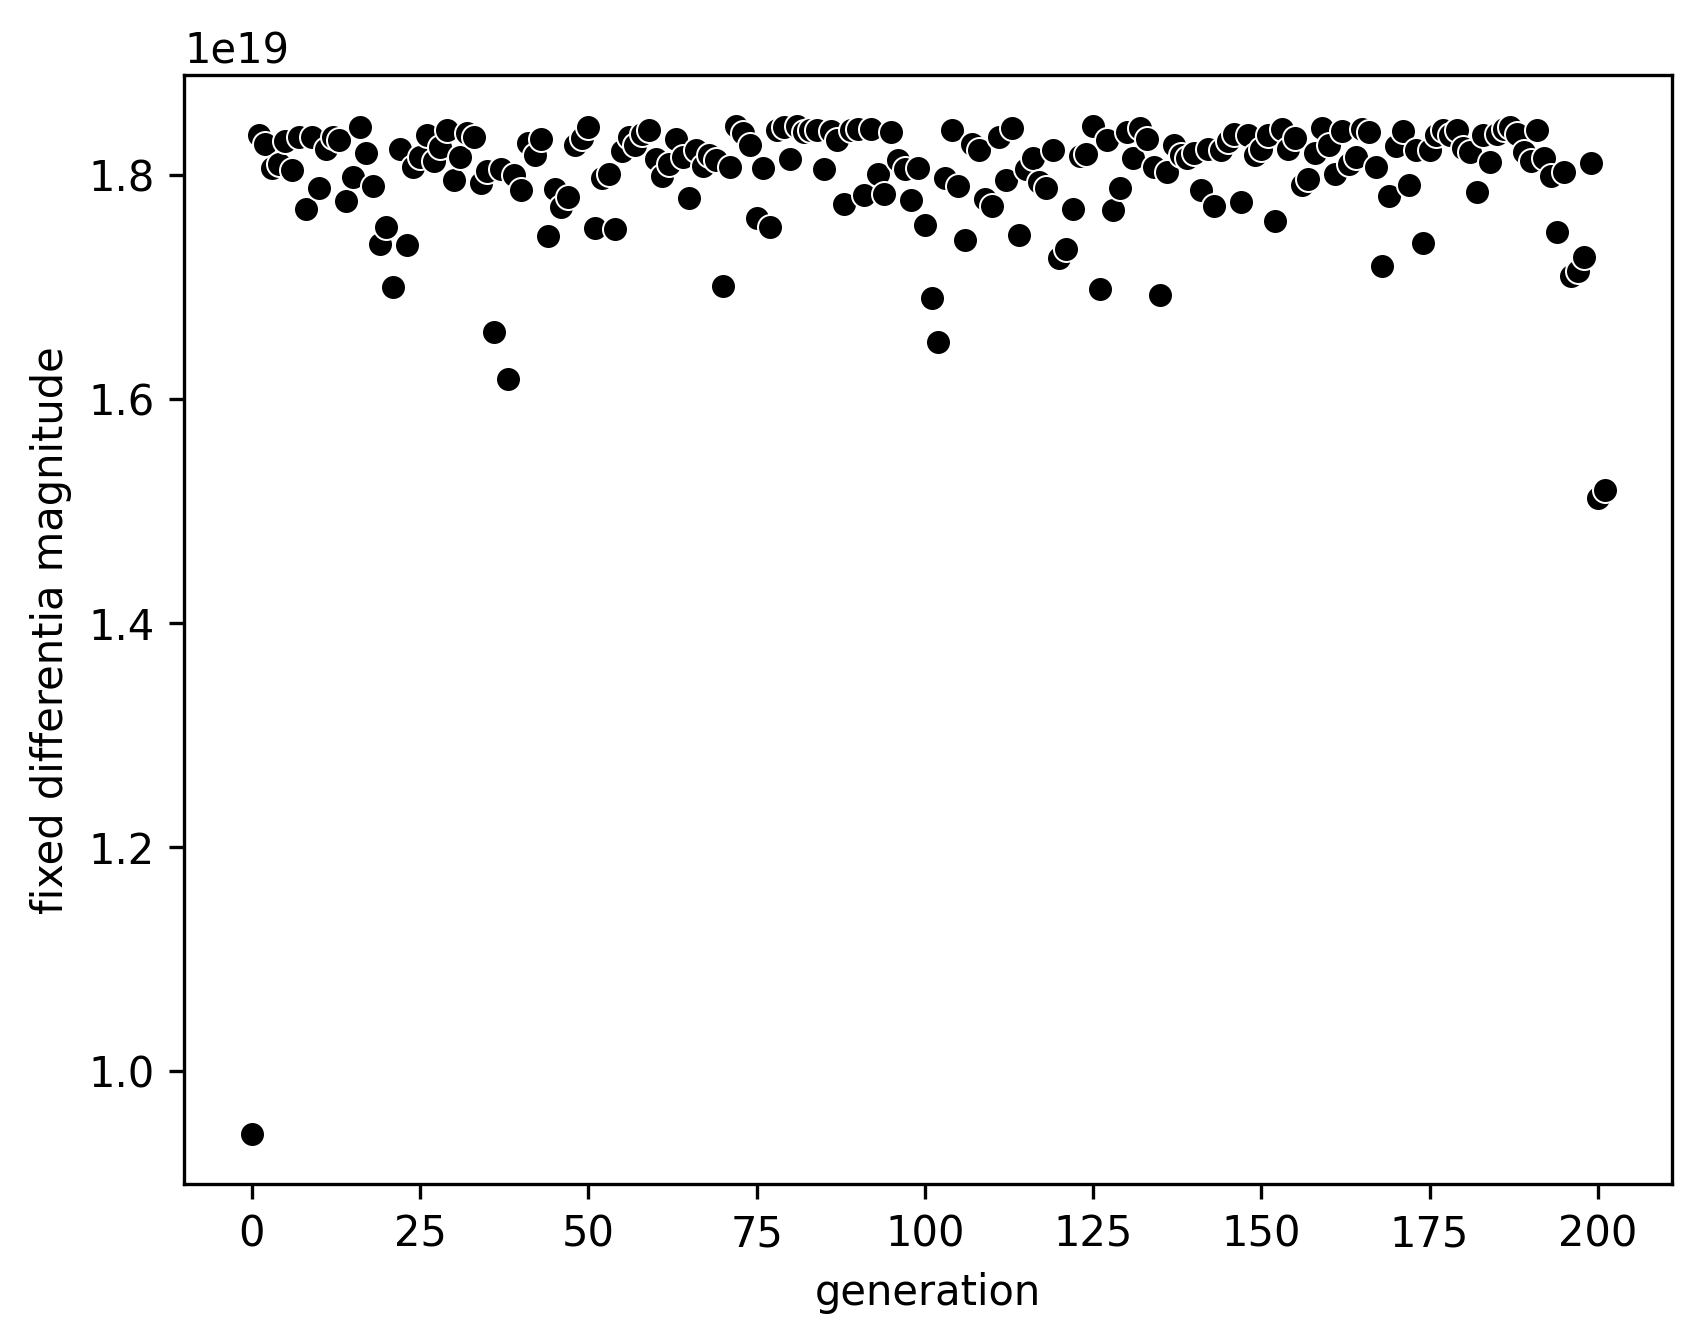
\includegraphics[height=0.25\textheight]{notebooks/notebooks/teeplots/notebook=ne-inference+replicate=0+treatment=control+viz=scatterplot-differentia-magnitude+ext=}
  \end{minipage}%
  \begin{minipage}{.25\textwidth}
    \subcaption{Fixed Species-level Differentia Magnitudes by Layer}
    \label{fig:ne-process-example:differentia}
  \end{minipage}

  \vspace{0.25em}

  \begin{minipage}{.65\textwidth}
    \centering
    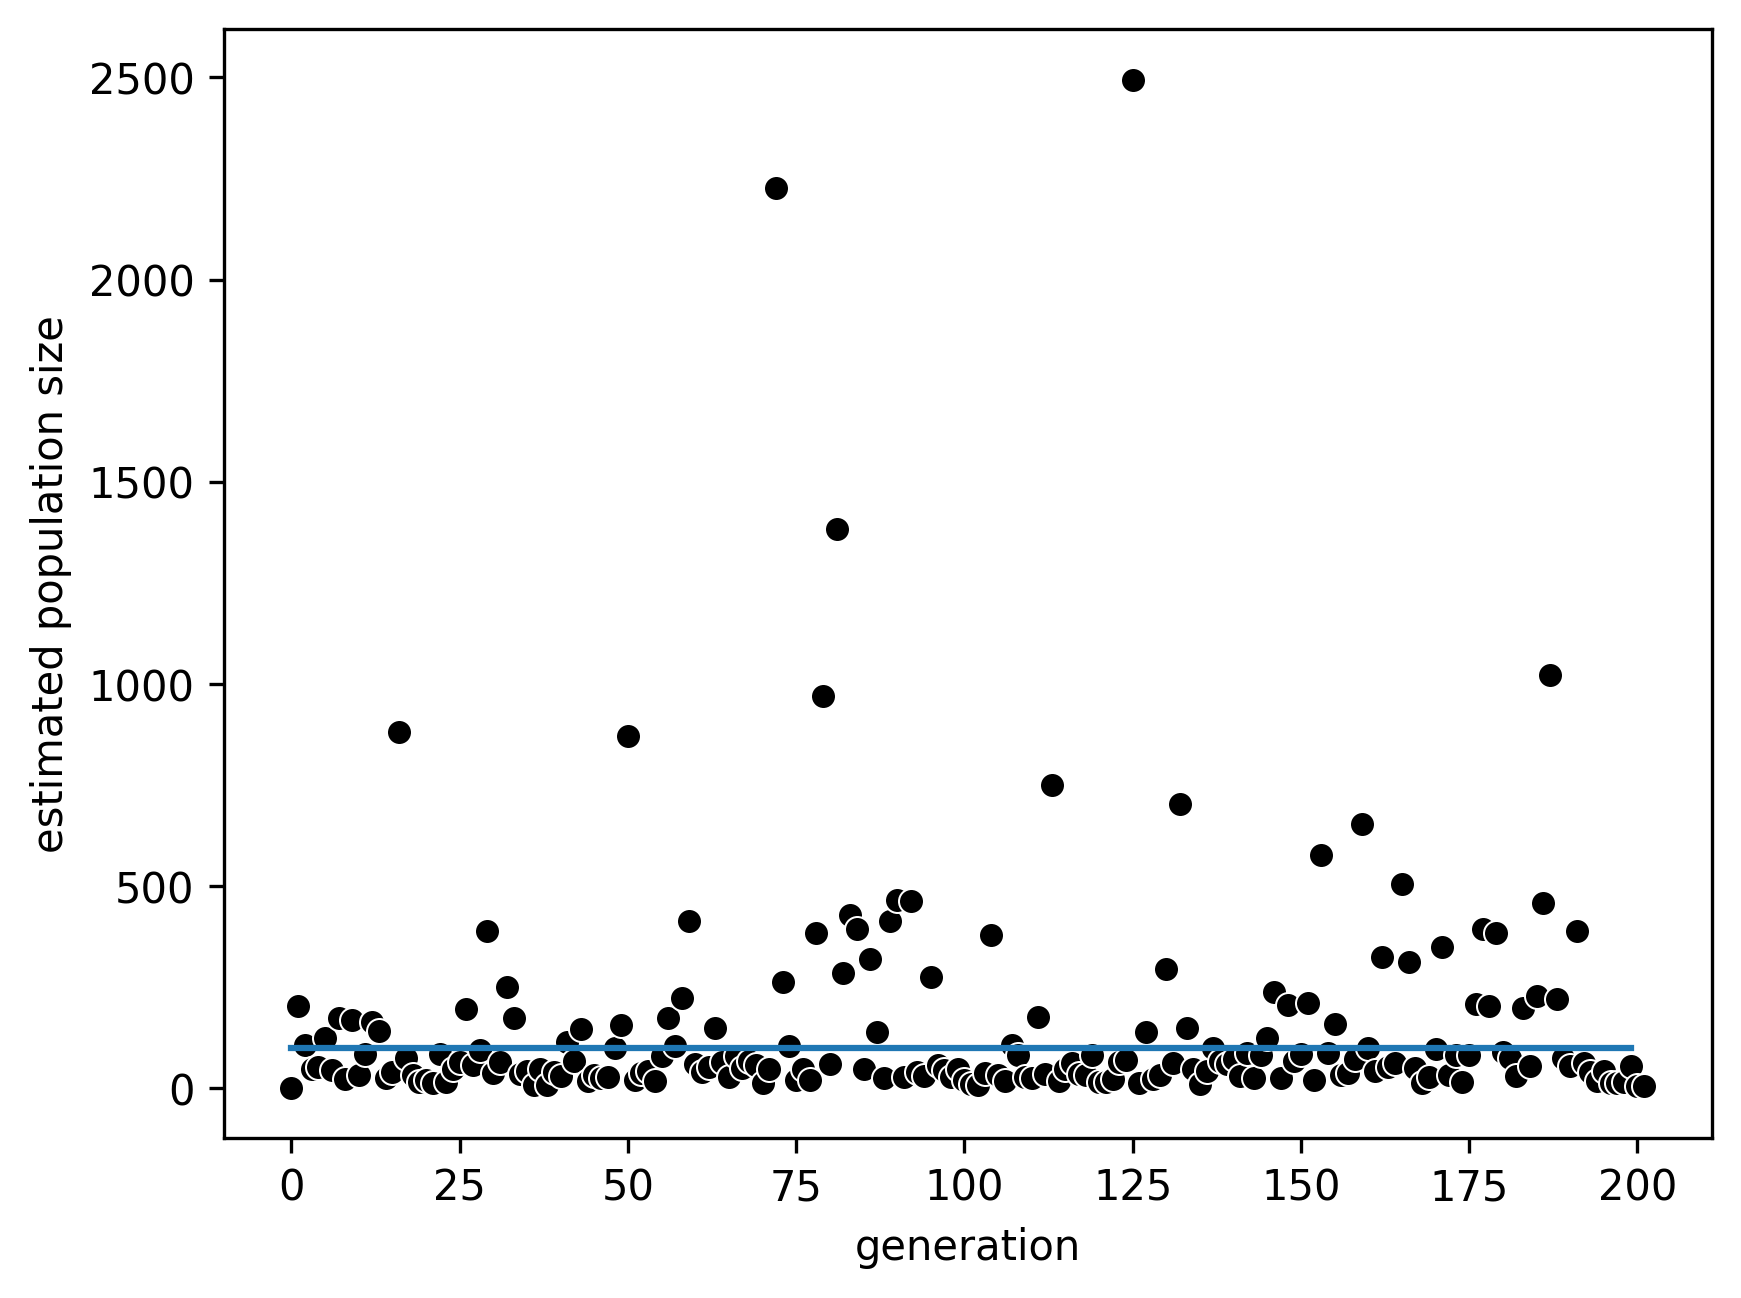
\includegraphics[height=0.25\textheight]{notebooks/notebooks/teeplots/notebook=ne-inference+replicate=0+treatment=control+viz=scatterplot-popsize-estimates+ext=}
  \end{minipage}%
  \begin{minipage}{.25\textwidth}
    \subcaption{Population Size Estimates}
    \label{fig:ne-process-example:singleton-est}
  \end{minipage}

  \vspace{0.25em}

  \begin{minipage}{.65\textwidth}
    \centering
    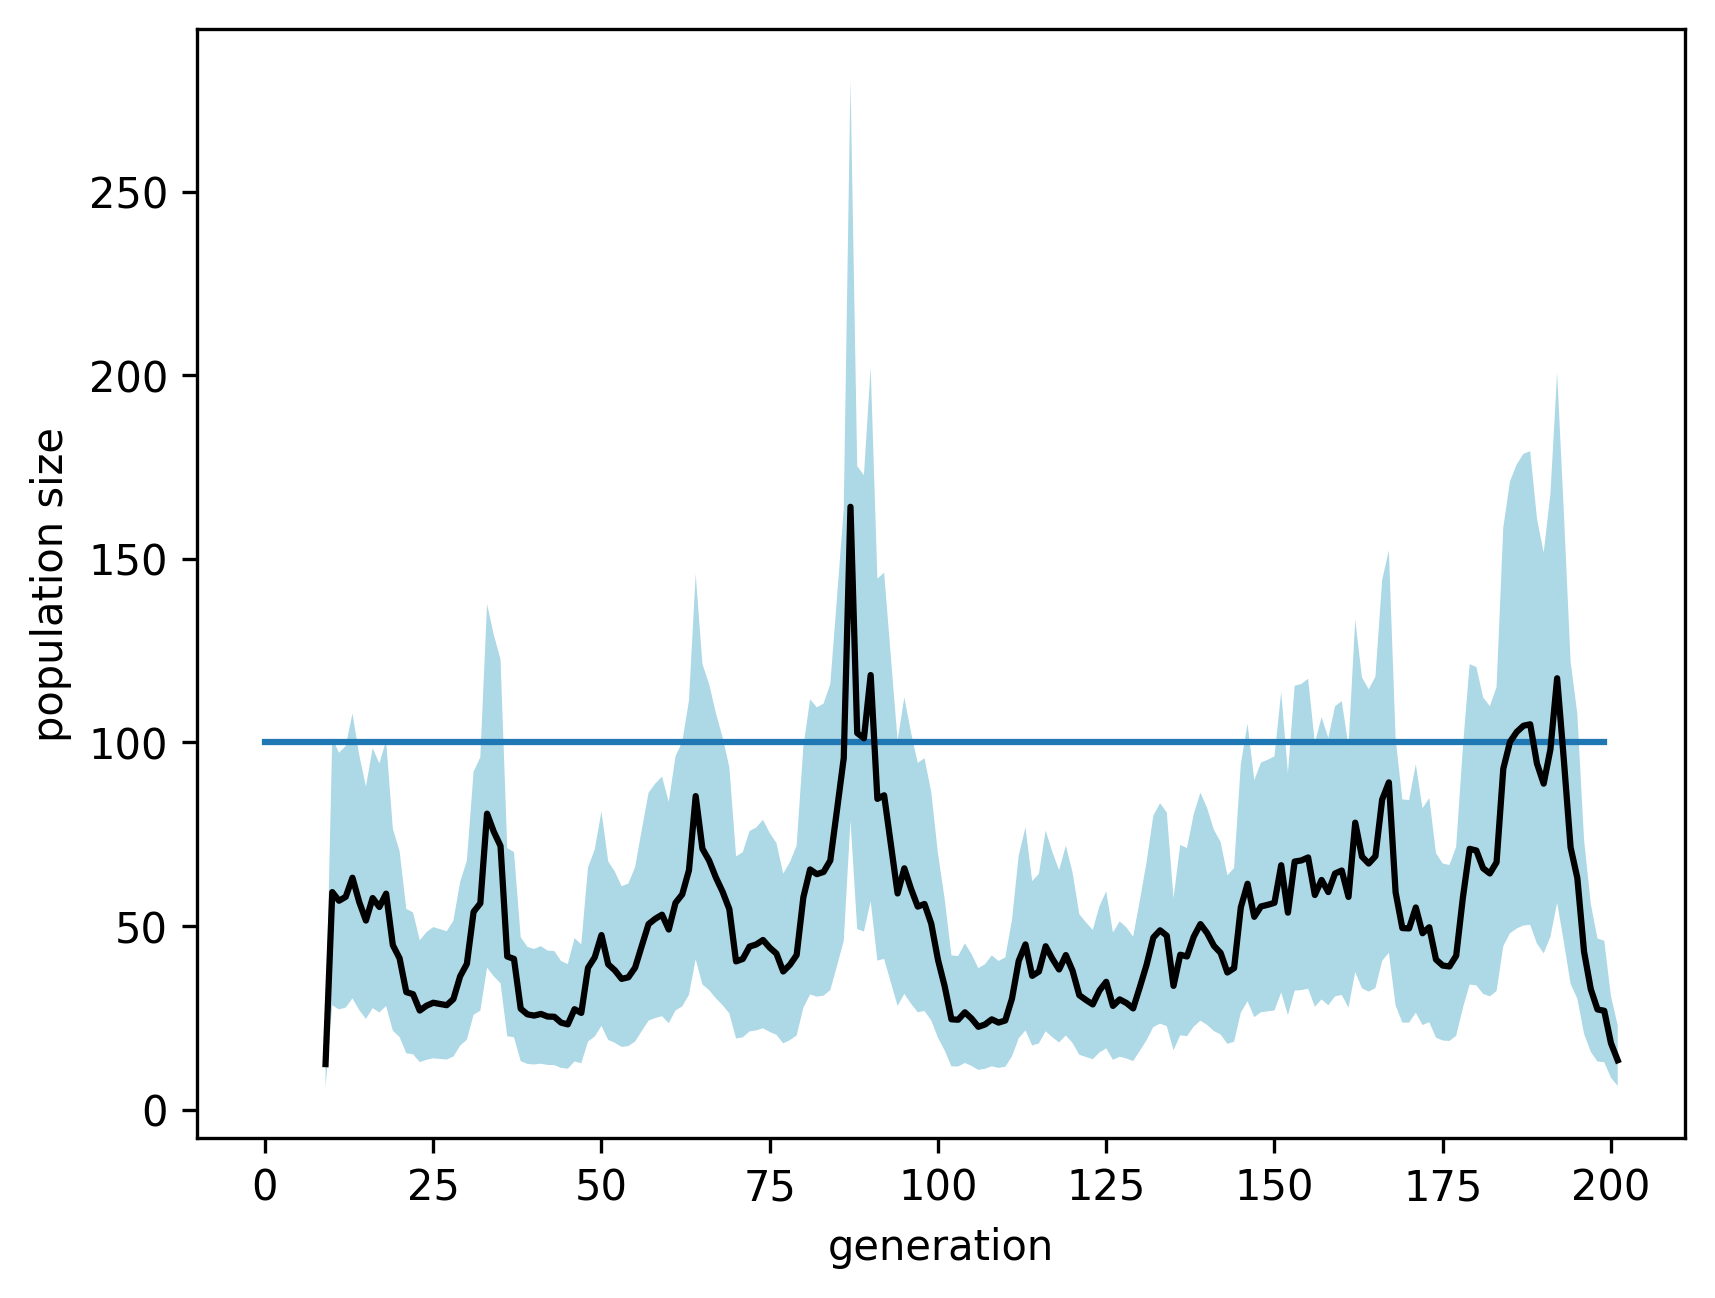
\includegraphics[height=0.25\textheight]{notebooks/notebooks/teeplots/notebook=ne-inference+replicate=0+treatment=control+viz=plot-running-estimation+x=rank+y=population-size+ext=}
  \end{minipage}%
  \begin{minipage}{.25\textwidth}
    \subcaption{Running Population Size Estimation with 95\% Confidence Intervals}
    \label{fig:ne-process-example:running-est}
  \end{minipage}

  \caption{
    Example population size estimation data.
    Differentia values are extracted from species-level annotation of a single extant population member (Subfigure \ref{fig:ne-process-example:differentia}).
    Subfigure \ref{fig:ne-process-example:singleton-est} shows one-off population size estimates at each generation from the corresponding differentia.
    To improve statistical informativeness, differentia values are grouped into a running pool of ten values to perform population size estimation.
    True population carrying capacity is annotated as a horizontal line.
    Note that systematic underestimation of ``carrying capacity'' population size is expected due to demographic factors excluding some population members from gene pool contributions.
    Figure \ref{fig:beta-explain} overviews the statistical mechanism used for population size distribution.
  }
  \label{fig:ne-process-example}
\end{figure}


% notebooks/notebooks/teeplots/notebook=ne-inference+replicate=0+treatment=control+viz=plot-running-estimation+x=rank+y=population-size+ext=.pdf
%
% notebooks/notebooks/teeplots/notebook=ne-inference+replicate=0+treatment=control+viz=scatterplot-differentia-magnitude+ext=.pdf
%
% notebooks/notebooks/teeplots/notebook=ne-inference+replicate=0+treatment=control+viz=scatterplot-popsize-estimates+ext=.pdf


% notebooks/notebooks/teeplots/notebook=ne-inference+replicate=0+treatment=bottleneck+viz=plot-running-estimation+x=rank+y=population-size+ext=.pdf
%
% notebooks/notebooks/teeplots/notebook=ne-inference+replicate=0+treatment=bottleneck+viz=scatterplot-differentia-magnitude+ext=.pdf
%
% notebooks/notebooks/teeplots/notebook=ne-inference+replicate=0+treatment=bottleneck+viz=scatterplot-popsize-estimates+ext=.pdf

% notebooks/notebooks/teeplots/notebook=ne-inference+replicate=0+treatment=range-expansion+viz=plot-running-estimation+x=rank+y=population-size+ext=.pdf
%
% notebooks/notebooks/teeplots/notebook=ne-inference+replicate=0+treatment=range-expansion+viz=scatterplot-differentia-magnitude+ext=.pdf
%
% notebooks/notebooks/teeplots/notebook=ne-inference+replicate=0+treatment=range-expansion+viz=scatterplot-differentia-magnitude+ext=.pdf
%
% notebooks/notebooks/teeplots/notebook=ne-inference+replicate=0+treatment=selection-pressure+viz=plot-running-estimation+x=rank+y=population-size+ext=.pdf
%
% notebooks/notebooks/teeplots/notebook=ne-inference+replicate=0+treatment=selection-pressure+viz=scatterplot-differentia-magnitude+ext=.pdf
%
% notebooks/notebooks/teeplots/notebook=ne-inference+replicate=0+treatment=selection-pressure+viz=scatterplot-popsize-estimates+ext=.pdf


Panel \ref{fig:ne-process-example:differentia} shows magnitudes of fixed differentia across the generational record extracted from a sample specimen at the end of the run.

Population size estimates can be computed at each generation using the maximum likelihood estimator (given in Equation \ref{eqn:popsize_mle}), as shown in Panel \ref{fig:ne-process-example:singleton-est}.
The true population size is annotated as a horizontal blue line.

To generate more robust inference, inference was pooled over rolling sets of 10 fixed differentia.
Population size estimates were again performed using the maximum likelihood estimator given in Equation \ref{eqn:popsize_mle} with confidence interval bounds computed via Equation \ref{eqn:popsize_mle_ci}.
Supplemental Figure \ref{fig:ne-process-example:running-est} plots this running estimation.
Note that some discrepancy is expected between absolute population size (horizontal line) and effective population size $N_e$ (estimated) due to demographic factors.



\subsection{Supplementary Figures}

\begin{SCfigure}[3][b]
  \centering
  \begin{subfigure}[b]{0.4\textwidth}
    \centering
    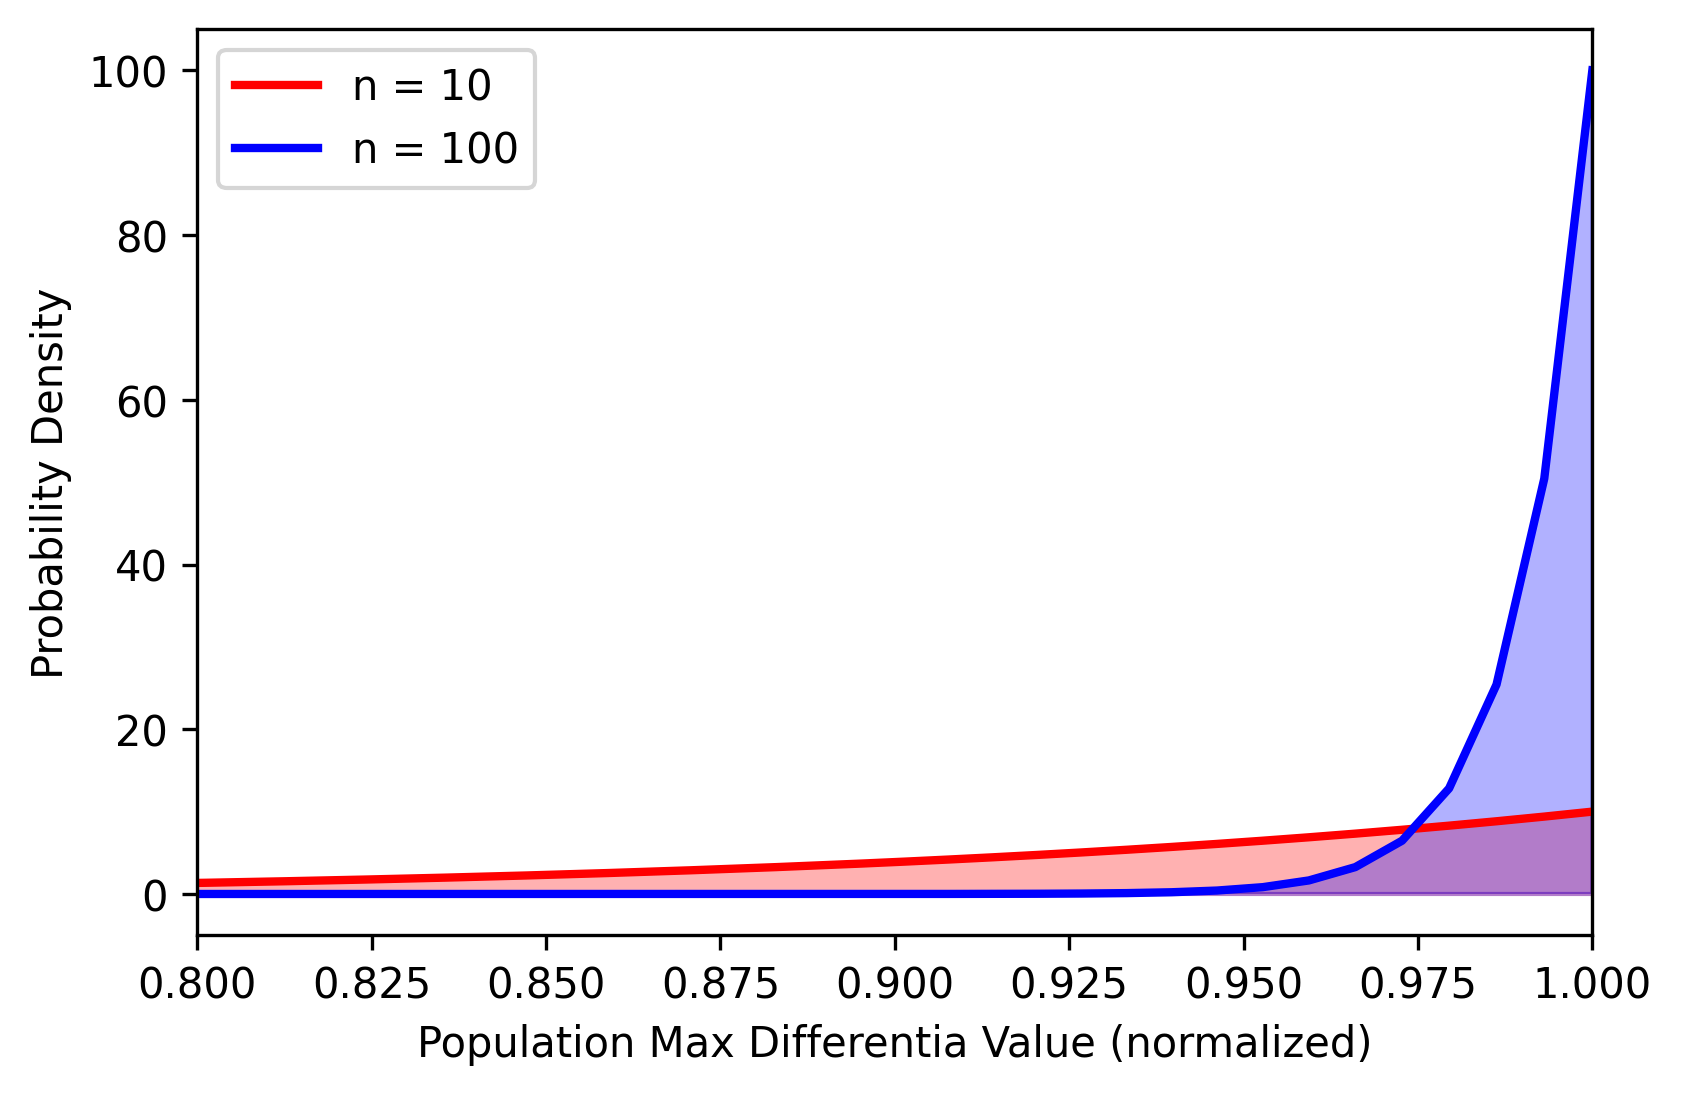
\includegraphics[width=\textwidth]{notebooks/notebooks/teeplots/viz=beta-pdf+ext=}
    % \caption{empty}
    % \label{fig:empty}
  \end{subfigure}%
  \begin{subfigure}[b]{0.25\textwidth}
    \centering
    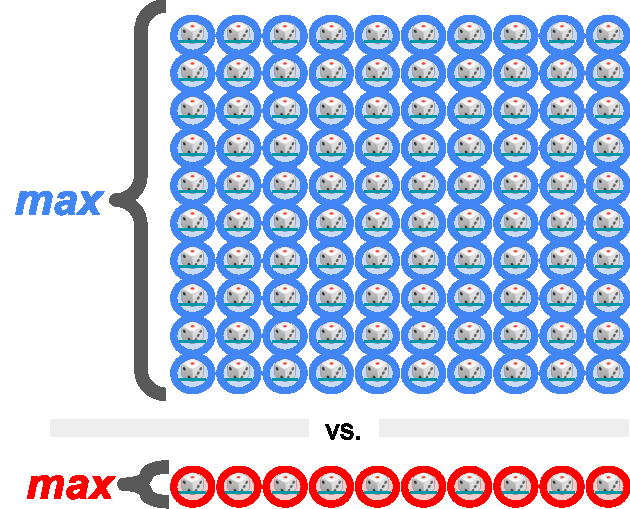
\includegraphics[width=\textwidth]{img/dice-pool}
    \vspace{2ex}
    % \caption{empty}
    % \label{fig:empty}
  \end{subfigure}
  \caption{
    Working principle of population size estimation.
    Increasing population size skews probability density function for population maximum value of generated fingerprints (referred to here as ``differentia'').
  }
  \label{fig:beta-explain}
\end{SCfigure}


\begin{SCfigure}[3]
  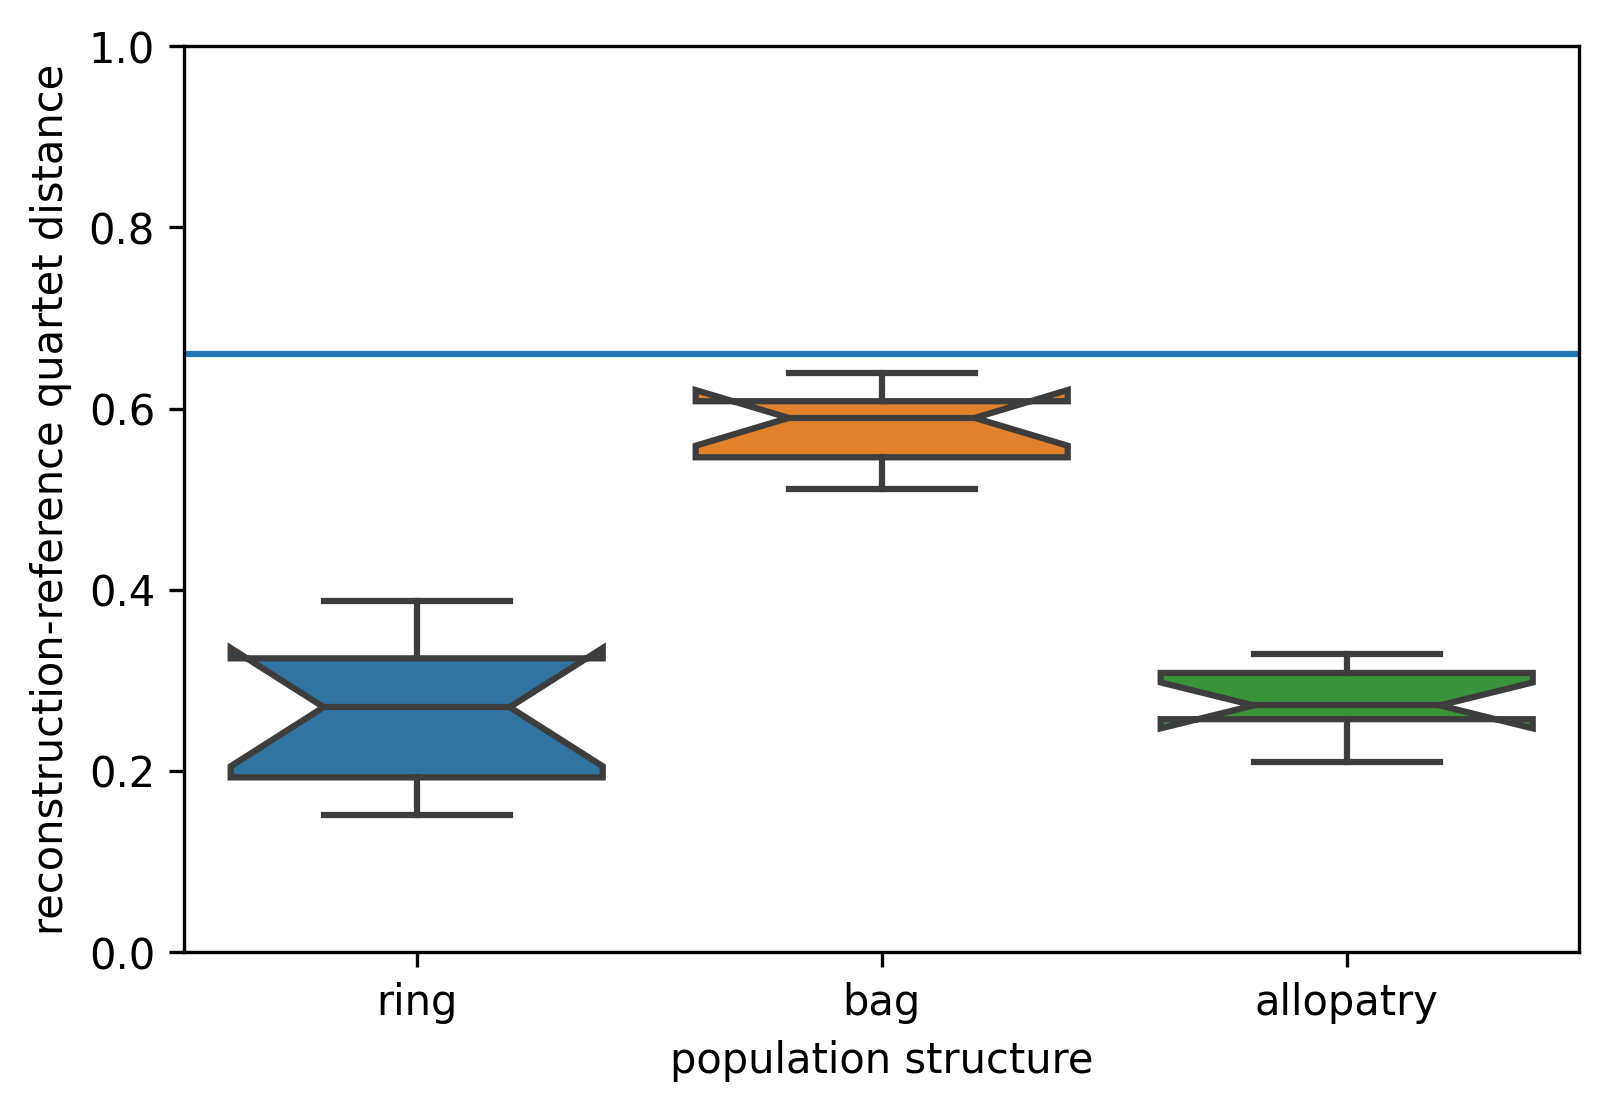
\includegraphics[width=0.5\textwidth]{notebooks/notebooks/teeplots/viz=boxplot-quartet+x=treatment+y=quartet-distance+ext=}
  \caption{
    Normalized quartet distances between reconstructed phylogenies and references distilled from tracked pedigree.
    Lower indicates less reconstruction error.
    Notches give bootstrapped 95\% CI.
    Horizontal blue line indicates expected quartet distance between random trees.
    Some reconstruction error is expected, especially in control treatment, due to resolution of effectively arbitrary phylogenetic structure among well-mixed population components.
  }
  \label{fig:species-reconstruction-error}
\end{SCfigure}


\begin{figure}
  \centering
  \begin{minipage}{\textwidth} % adjust the width as needed

    \begin{minipage}{0.5\textwidth}
      \centering
      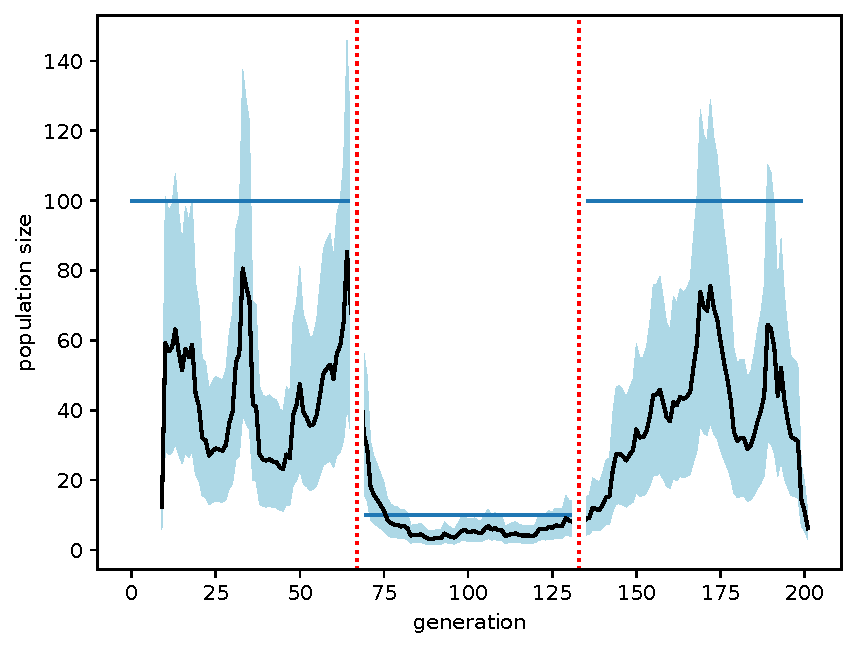
\includegraphics[height=0.23\textheight]{notebooks/notebooks/teeplots/notebook=ne-inference+replicate=0+treatment=bottleneck+viz=plot-running-estimation+x=rank+y=population-size+ext=}
      \subcaption{Bottleneck treatment}
      \label{fig:ne-example-replicates:bottleneck}
    \end{minipage}%
    \begin{minipage}{0.5\textwidth}
      \centering
      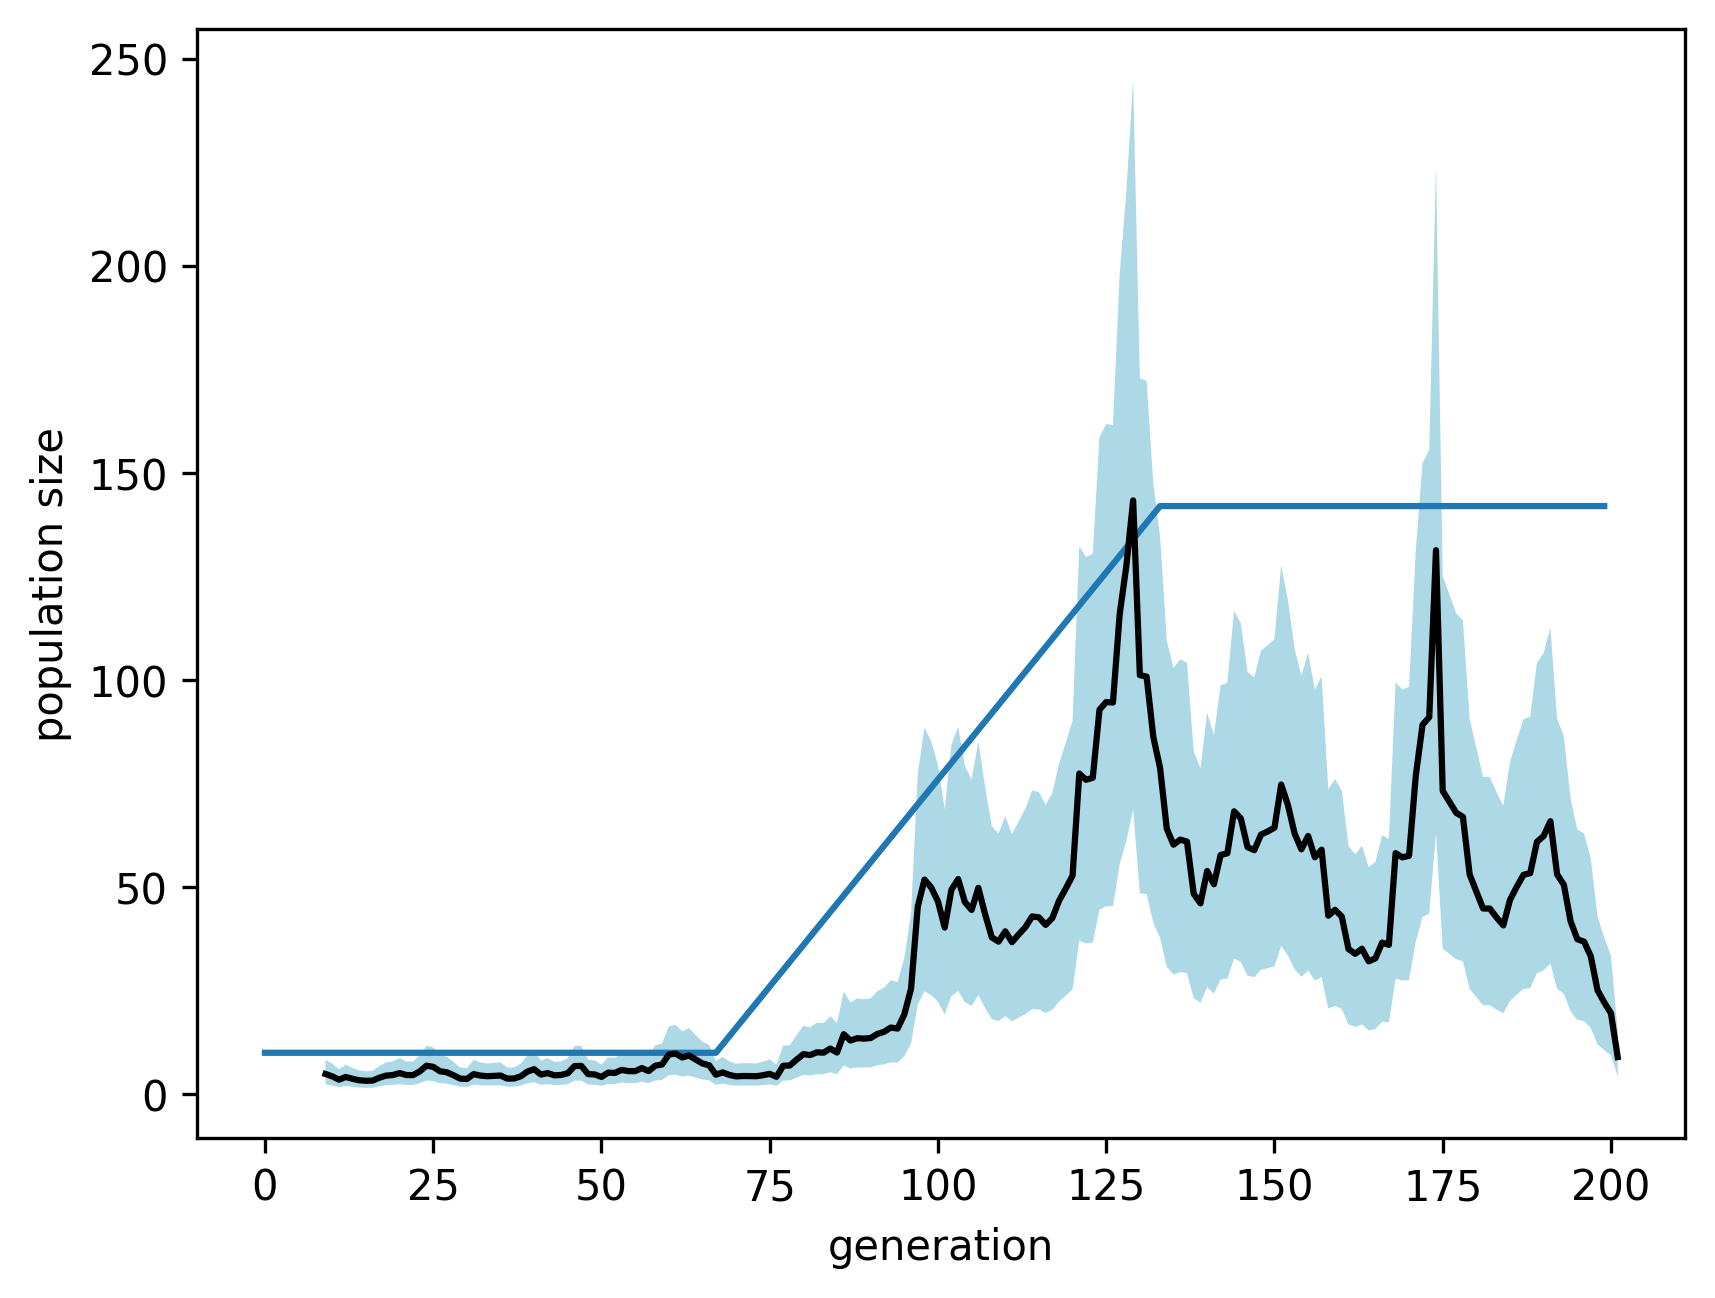
\includegraphics[height=0.23\textheight]{notebooks/notebooks/teeplots/notebook=ne-inference+replicate=0+treatment=range-expansion+viz=plot-running-estimation+x=rank+y=population-size+ext=}
      \subcaption{Range expansion treatment}
      \label{fig:ne-example-replicates:range_expansion}
    \end{minipage}

    \begin{minipage}{0.5\textwidth}
      \centering
      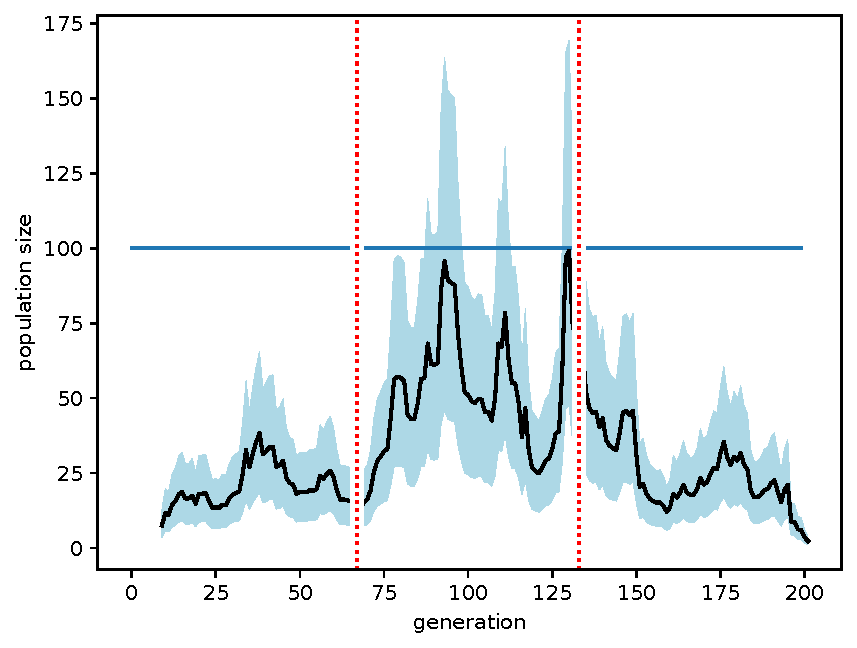
\includegraphics[height=0.23\textheight]{notebooks/notebooks/teeplots/notebook=ne-inference+replicate=0+treatment=selection-pressure+viz=plot-running-estimation+x=rank+y=population-size+ext=}
      \subcaption{Selection pressure treatment}
      \label{fig:ne-example-replicates:selection_pressure}
    \end{minipage}%
    \begin{minipage}{0.5\textwidth}
      \centering
      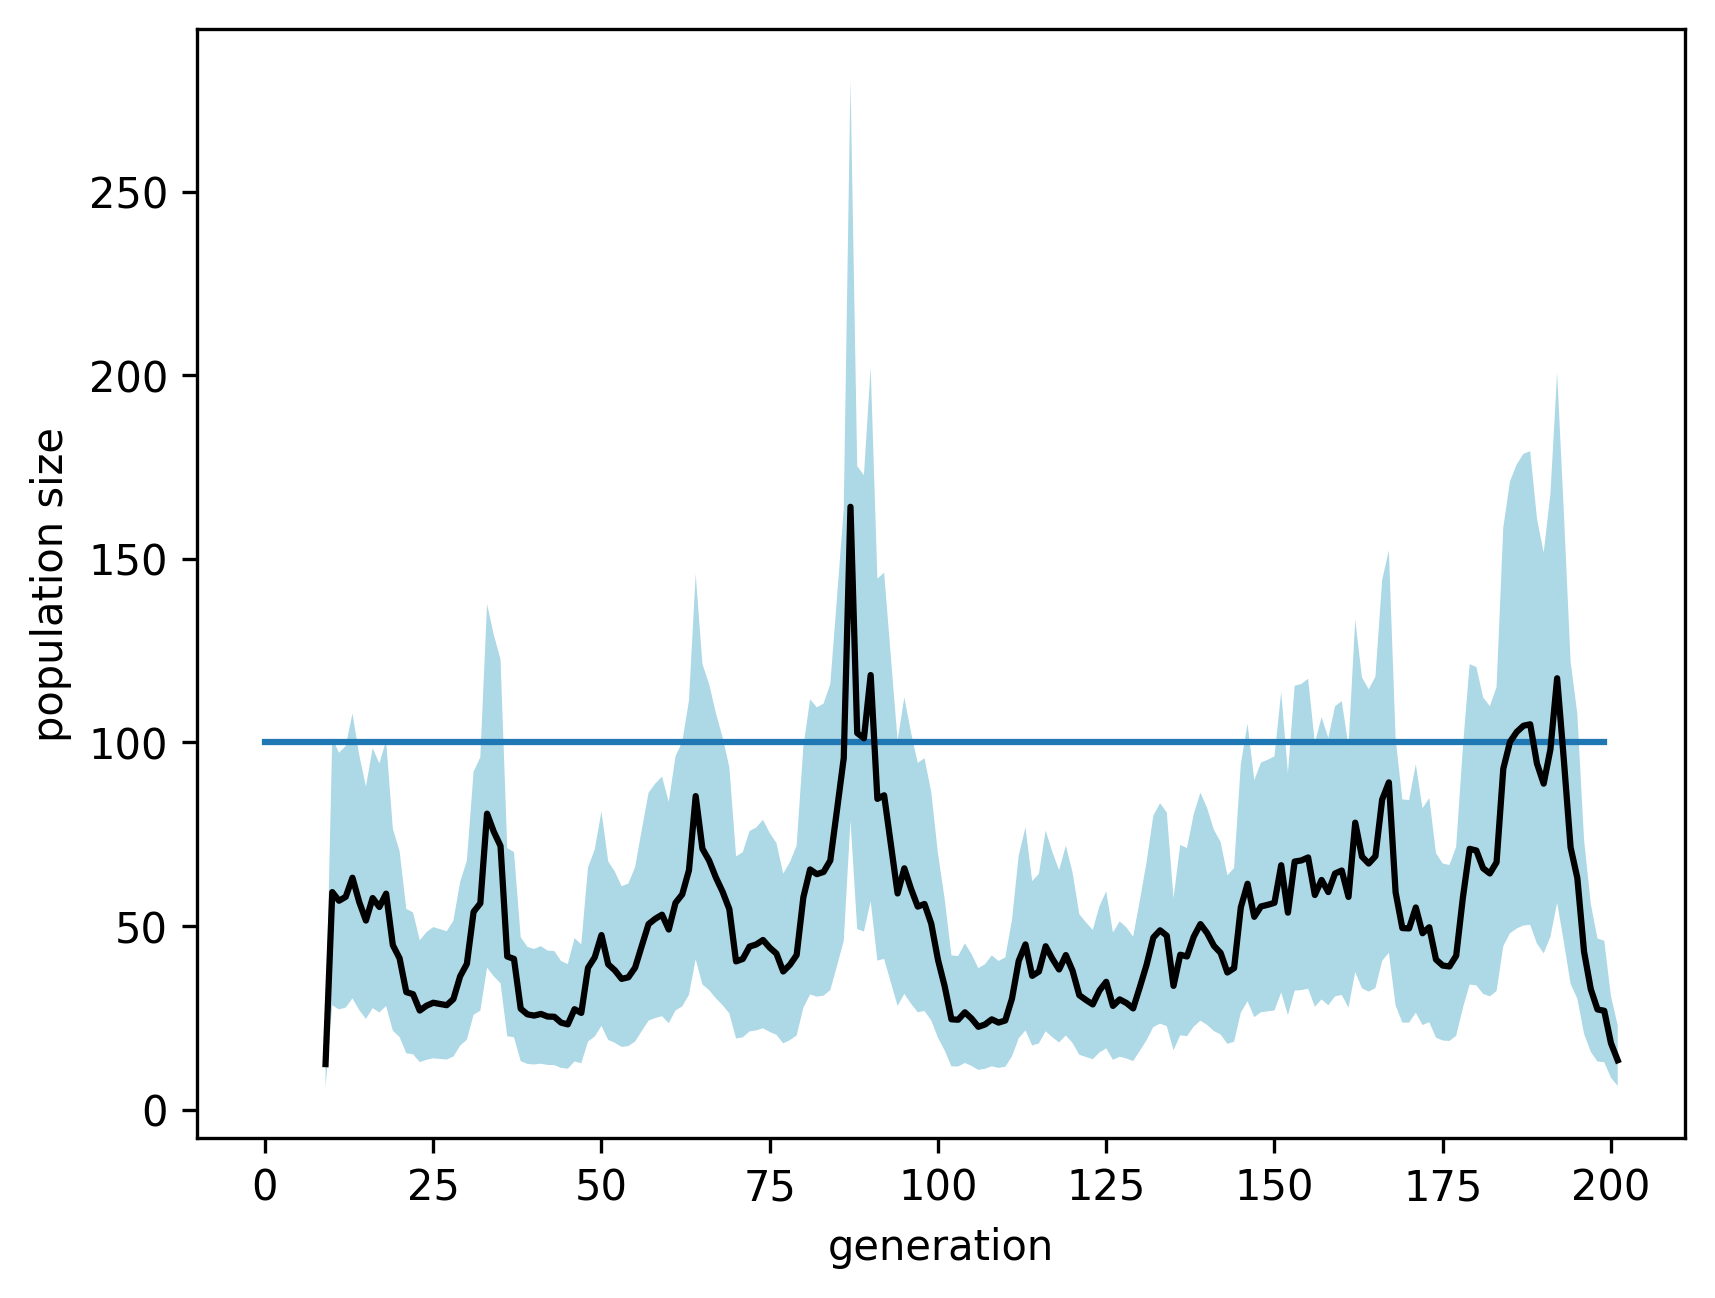
\includegraphics[height=0.23\textheight]{notebooks/notebooks/teeplots/notebook=ne-inference+replicate=0+treatment=control+viz=plot-running-estimation+x=rank+y=population-size+ext=}
      \subcaption{Control treatment}
      \label{fig:ne-example-replicates:control}
    \end{minipage}

  \end{minipage}
  \hfill % Creates horizontal space. Can also use \hspace{<len>}
  \begin{minipage}{\textwidth} % adjust the width as needed
    \vspace{2ex}
    \caption{Ten-sample running MLE estmate of effective population size of example replicates from  each treatment.
    Shaded region corresponds to 95\% MLE confidence interval.
    Horizontal blue lines indicate true population size.
    Dashed vertical lines indicate treatment discontinuities.
    See Section \ref{sec:population-size-inference-experiments} for population size and selection pressure manipulations performed for each treatment.
    Note that disparity between estimated effective population size and true population size is expected due to demographic factors depressing effective population size.
    }
    \label{fig:ne-example-replicates}
  \end{minipage}

\end{figure}


% notebooks/notebooks/teeplots/notebook=ne-inference+replicate=0+treatment=bottleneck+viz=plot-running-estimation+x=rank+y=population-size+ext=.pdf
%
% notebooks/notebooks/teeplots/notebook=ne-inference+replicate=0+treatment=control+viz=plot-running-estimation+x=rank+y=population-size+ext=.pdf
%
% notebooks/notebooks/teeplots/notebook=ne-inference+replicate=0+treatment=range-expansion+viz=plot-running-estimation+x=rank+y=population-size+ext=.pdf
%
% notebooks/notebooks/teeplots/notebook=ne-inference+replicate=0+treatment=selection-pressure+viz=plot-running-estimation+x=rank+y=population-size+ext=.pdf


\begin{figure}
  \centering

  \begin{subfigure}{\textwidth}
    \begin{minipage}{0.7\textwidth}
      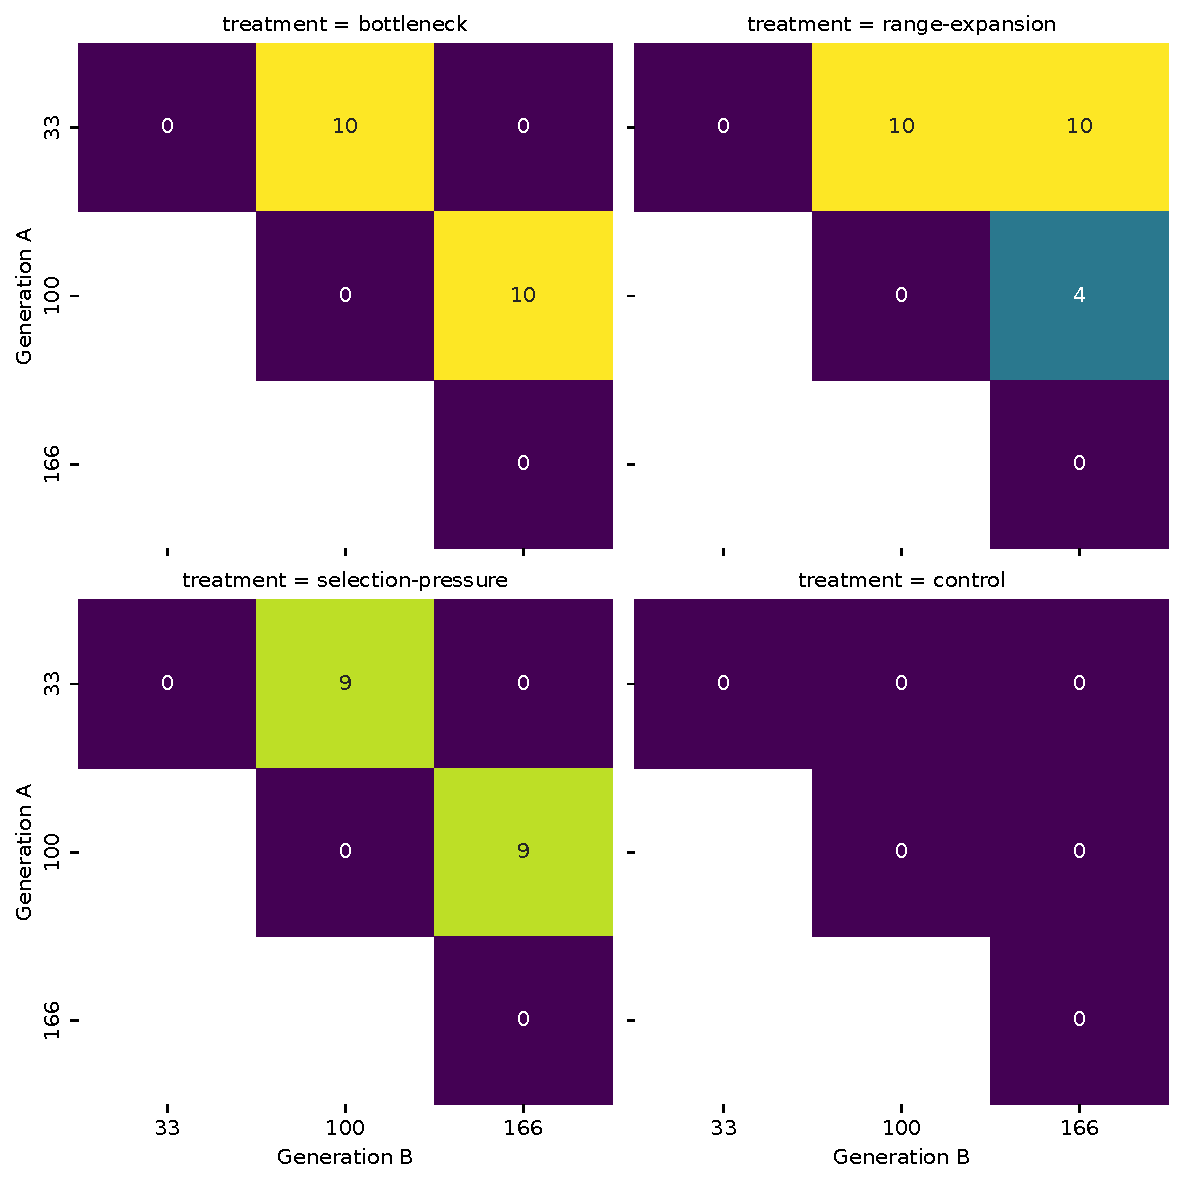
\includegraphics[width=\linewidth]{notebooks/notebooks/teeplots/hue=mann-whitney-significant-at-alpha-0-01+viz=facet-heatmap+x=generation-b+y=generation-a+ext=}
    \end{minipage}%
    \begin{minipage}{0.25\textwidth}
      \caption{Mann-Whitney comparison of 33 annotations at time points surrounding each target generation, with significance threshold $\alpha = 0.01$.}
      \label{fig:ne-detection-matrix:mann-whitney}
    \end{minipage}
  \end{subfigure}

  \vspace{1em} % adjust the vertical spacing between the subfigures

  \begin{subfigure}{\textwidth}
    \begin{minipage}{0.7\textwidth}
      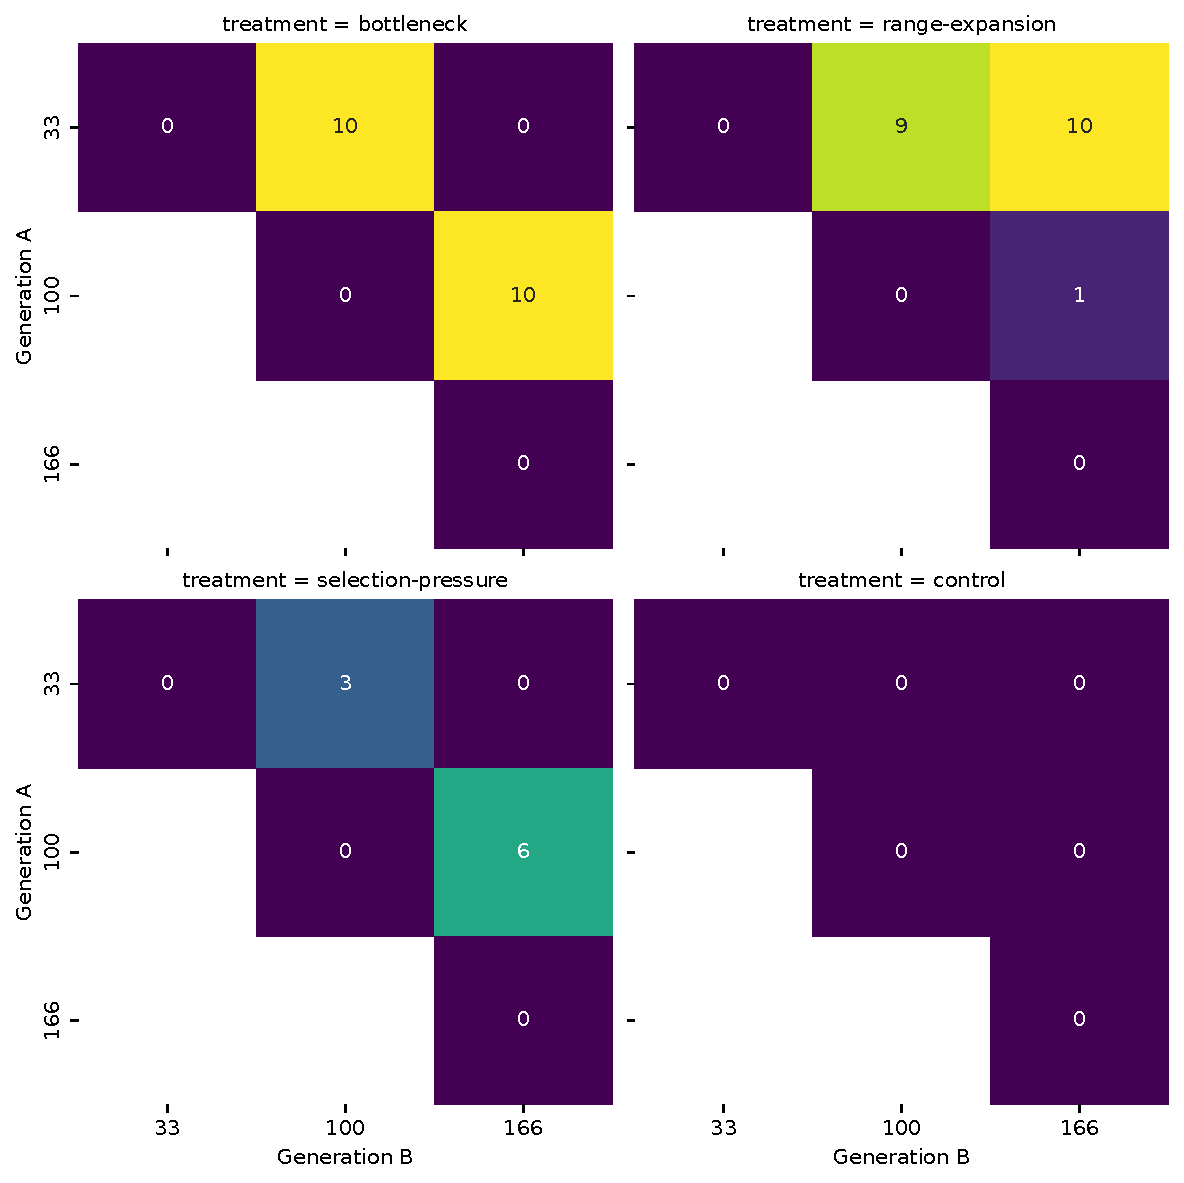
\includegraphics[width=\linewidth]{notebooks/notebooks/teeplots/hue=nonoverlapping-ci+viz=facet-heatmap+x=generation-b+y=generation-a+ext=}
    \end{minipage}%
    \begin{minipage}{0.25\textwidth}
      \caption{Non-overlapping MLE 95\% confidence intervals for rolling 10-sample estimate at target generations.}
      \label{fig:ne-detection-matrix:ci}
    \end{minipage}
  \end{subfigure}

  \caption{Counts of replicates where significant differences in effective population size ($N_e$) were detected between time point pairs.
  Counts are out of 10 total replicates attempted.
  All time point pairs had true differences in $N_e$, except same-time point pairs and time point pairs in the control experiment (Section \ref{sec:population-size-inference-experiments}.
  }
  \label{fig:ne-detection-matrix}
\end{figure}

% notebooks/notebooks/teeplots/hue=mann-whitney-significant-at-alpha-0-01+viz=facet-heatmap+x=generation-b+y=generation-a+ext=.pdf
%
% notebooks/notebooks/teeplots/hue=nonoverlapping-ci+viz=facet-heatmap+x=generation-b+y=generation-a+ext=.pdf


\begin{figure}
  \centering
  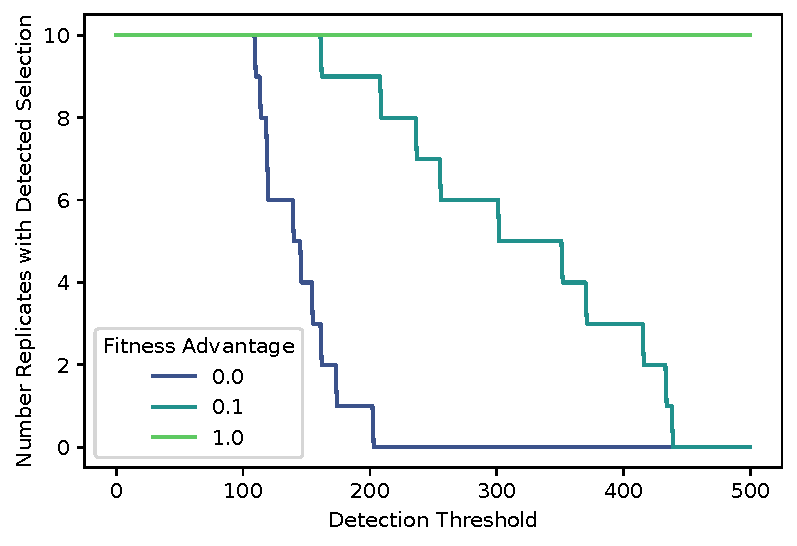
\includegraphics[width=0.8\textwidth]{notebooks/notebooks/teeplots/hue=fitness-advantage+viz=lineplot-detection+x=threshold+y=replicate-count+ext=}
  \caption{
    Gene selection detection rates by threshold for each fitness advantage level among 10 replicates.
    Fitness advantage 0.0 inferred no selective benefit, so all selection detections on this treatment are false positives.
    Detection threshold 200 distinguishes treatment 0.0 and 0.1 with one false positive and one false negative.
  }
  \label{fig:selection-sensitivity-specificity}
\end{figure}


% \section{Example} \label{sec:example}

example \citep{gropp1996high}

